\apendice{Documentación técnica de programación}

\section{Introducción}
En esta sección se explica la estructura del proyecto, el proceso de instalación del framework y herramientas necesarias para desarrollar el trabajo, cómo realizar la compilación, instalación y ejecución del proyecto y las pruebas que se han llevado a cabo.

\section{Estructura de directorios}

\section{Manual del programador}
A continuación se explicará cómo realizar la instalación de los programas necesarios para el desarrollo de la aplicación.

\subsection{Instalación de Java}
Como en el proyecto se usa Vaadin 8 se debe emplear la versión 8 de Java, es decir, JDK 8. Para descargar JDK 8 se deberá ir a la \href{https://www.oracle.com/java/technologies/javase/javase-jdk8-downloads.html}{página de descargas de Oracle Java SE 8.0} y descargar la versión correspondiente para tu sistema operativo.

\imagen{Descarga_JDK_8}{Descarga de JDK 8}

Una vez descargado, se deberá ejecutar el instalador y seguir el proceso de instalación del asistente.

\subsection{Instalación de Eclipse}
Lo siguiente será instalar un entorno de desarrollo integrado(IDE) para Java, en este caso se ha utilizado \textbf{Eclipse IDE for Enterprise Java Developers} en la versión 2020-06. 

Para descargar el IDE se accederá a la \href{https://www.eclipse.org/downloads/packages/release/2020-06/r}{página de descargas de Eclipse} y descargar la opción correspondiente a nuestro sistema operativo del ``\textbf{\textit{Eclipse IDE for Enterprise Java Developers}}''.
\imagen{Descargar_IDE_Eclipse}{Descargar IDE Eclipse}

Tras esto, se debe ejecutar el instalador que se ha descargado y continuar el proceso a través del asistente.

\subsection{Instalación del \textit{plugin} de Vaadin para Eclipse}
Una vez se haya instalado Eclipse, se procederá a añadir el plugin de Vaadin para Eclipse. 
Esto se realizará mediante el Eclipse Marketplace de Eclipse, el cual se encuentra en la opción de Help de la barra de herramientas. 
\imagen{Eclipse_marketplace}{Eclipse marketplace}

Una vez en el Eclipse Marketplace', se buscará vaadin y aparecera el plugin con nombre Vaadin Plugin for Eclipse, se dará a install y comenzará la instalación del plugin. Ver imagen \ref{img:Vaadin}.

\begin{figure}
\centering
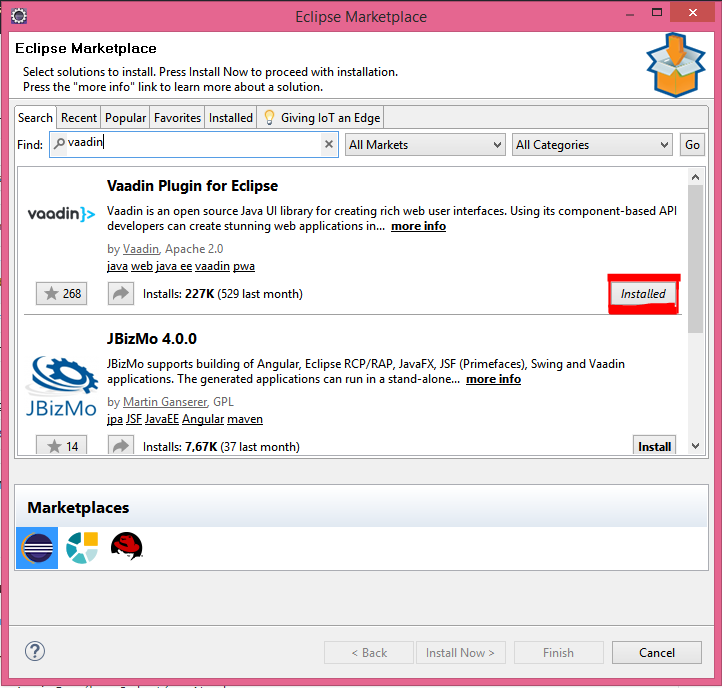
\includegraphics[width=0.5\textwidth]{img/Plugin_Vaadin}
\caption{Plugin Vaadin}\label{img:Vaadin}
\end{figure}

\section{Compilación, instalación y ejecución del proyecto}
Se explicará como compilar, instalar e ejecutar el proyecto. En el caso de la ejecución, se detallará como hacerlo con el términal de Windows y mediante Eclipse (IDE).

\subsection{Descarga del código fuente}
El código fuente se encuentra en el \href{https://github.com/dbo1001/Gestor-TFG-2016}{repositorio del proyecto} en GitHub. Para descargarlo se deberá hacer click en ``\textbf{\textit{Code}}'' y copiar la URL que se enseña en el apartado de HTTP. Con esta URL deberemos ir al GitHub Desktop y clonar el repositorio.

\imagen{GitHub_Code}{Copiar URL repositorio}

Para tener el código en local se deberá descargar el zip  ``\textbf{\textit{Download ZIP}}'' en la opción ``\textbf{\textit{Code}}'' anteriormente mencionada. Una vez descargado el zip se descomprimirá y abrirá con Eclipse. 
Para abrir el proyecto con eclipse se seleccionara en la barra de herramientas \textbf{\textit{File/Import\dots}}. Aparecerá una ventana en la que se optará por la opción ``\textbf{\textit{Projects from Folder or Archieve}}'' y se hará click en ``\textbf{\textit{Next}}''.

Después se hará click en ``\textbf{\textit{Directory\dots}}'' y se seleccionará la carpeta del proyecto con nombre sistinf y términaremos la importación con ``\textbf{\textit{Finish}}''.

\section{Pruebas del sistema}
